%%%% CAPÍTULO 3 - MATERIAL E MÉTODOS (PODE SER OUTRO TÍTULO DE ACORDO COM O TRABALHO REALIZADO)

\chapter{Metodologia}\label{cap:metodologia}

A metodologia utilizada neste projeto é a experimentação. Com base nisso, a
abordagem proposta baseia-se no desenvolvimento de um mecanismo de versionamento
diferencial otimizado para arquivos \gls{glb}, fundamentado na fragmentação do
binário em blocos lógicos. Utilizando a estrutura de \textit{bufferViews} do
\gls{gltf} como critério de segmentação, a abordagem permite identificar e armazenar
apenas as seções que sofreram alterações, como geometria ou animações, em vez de
replicar o arquivo integralmente. Essa estratégia aproveita a arquitetura modular do
formato para reduzir a redundância nos repositórios, visando validar a eficiência do
versionamento por blocos em termos de economia de armazenamento e desempenho
sistêmico. A Figura~\ref{fig:fluxo-glb} ilustra o fluxo geral de como o \gls{glb} é
tratado no método, e é explicada mais detalhadamente ao longo desta seção.

\begin{figure}[htb]
  \centering
  \caption{\label{fig:fluxo-glb}Fluxo de observação do arquivo}
  \fbox{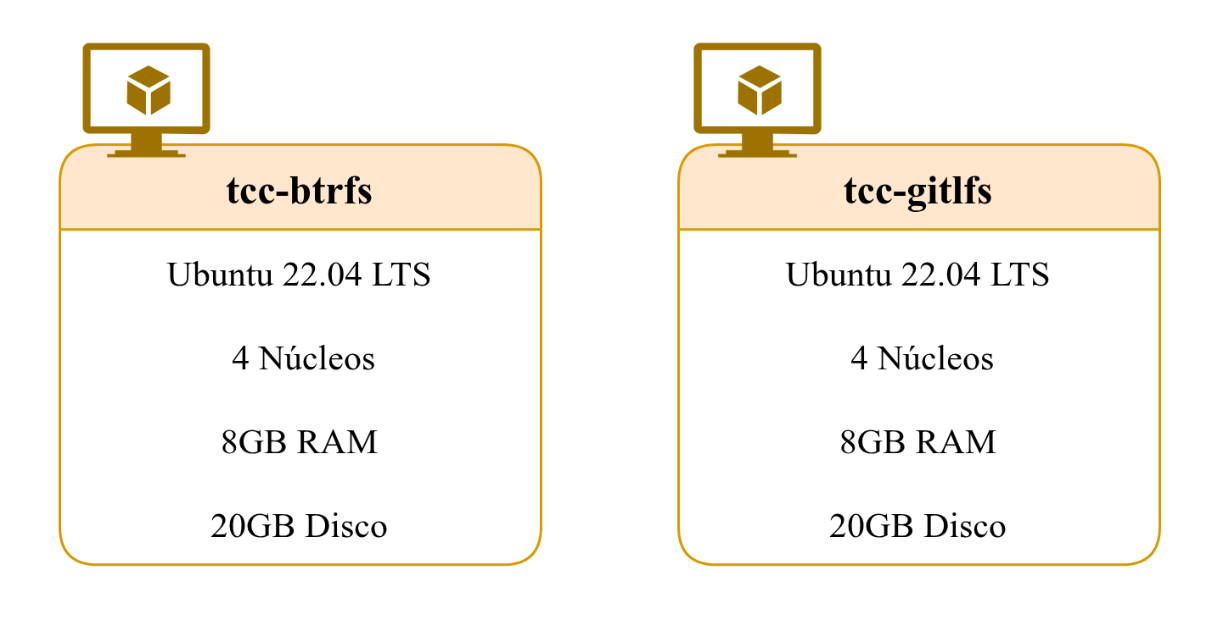
\includegraphics[width=0.8\textwidth]{figuras/maquinas-virtuais.png}}
  \fonte{Autoria própria (2026)}
\end{figure}

Para a implementação do algoritmo de segmentação e análise dos arquivos \gls{glb},
utiliza-se a linguagem Python com os módulos nativos \texttt{struct} e
\texttt{json}, responsáveis respectivamente pela leitura dos binários do contêiner
\gls{glb} e pela interpretação da estrutura \gls{json} que descreve as
\textit{bufferViews} do modelo. Complementarmente, o \gls{gitlfs} é configurado na
segunda instância para servir como método de referência, permitindo medir a eficácia
da abordagem proposta em relação a um padrão de versionamento consolidado na
indústria. Os modelos tridimensionais utilizados nos testes provêm do repositório
oficial de amostras do Khronos Group \cite{KhronosSamples2026}.

\section{Procedimentos Experimentais}

Os procedimentos experimentais são organizados de forma a permitir uma comparação direta e controlada entre a abordagem proposta e o método de referência. Para isso, ambos os ambientes recebem o mesmo modelo tridimensional como entrada e são submetidos ao mesmo conjunto de versões modificadas, geradas com parâmetros idênticos e reproduzíveis. A seguir são descritos o objeto de teste selecionado, o processo de geração controlada das versões, o fluxo de execução de cada método e as métricas utilizadas para avaliação dos resultados.

\subsection{Objeto de teste}

A escolha do modelo tridimensional \texttt{ABeautifulGame.glb} como objeto de teste
para este estudo fundamenta-se nas características que o tornam particularmente
adequado para o versionamento por blocos, conforme delineado na
Seção~\ref{sec:desafios-binarios} do referencial teórico. O modelo atende aos critérios
de um \textit{layout} previsível e de uma segmentação interna bem definida por
\textit{bufferViews}, característica essencial para a aplicação eficiente de
estratégias de armazenamento diferencial. Adicionalmente, o modelo não possui
compressão global nem criptografia, fatores que comprometem a granularidade e a
eficácia do versionamento baseado em blocos \cite{MacDonald2000}. O modelo
selecionado pode ser observado na Figura~\ref{fig:abeautifulgame}.

\begin{figure}[htb]
  \centering
  \caption{\label{fig:abeautifulgame}Cena tridimensional disponibilizada pelo Khronos Group}
  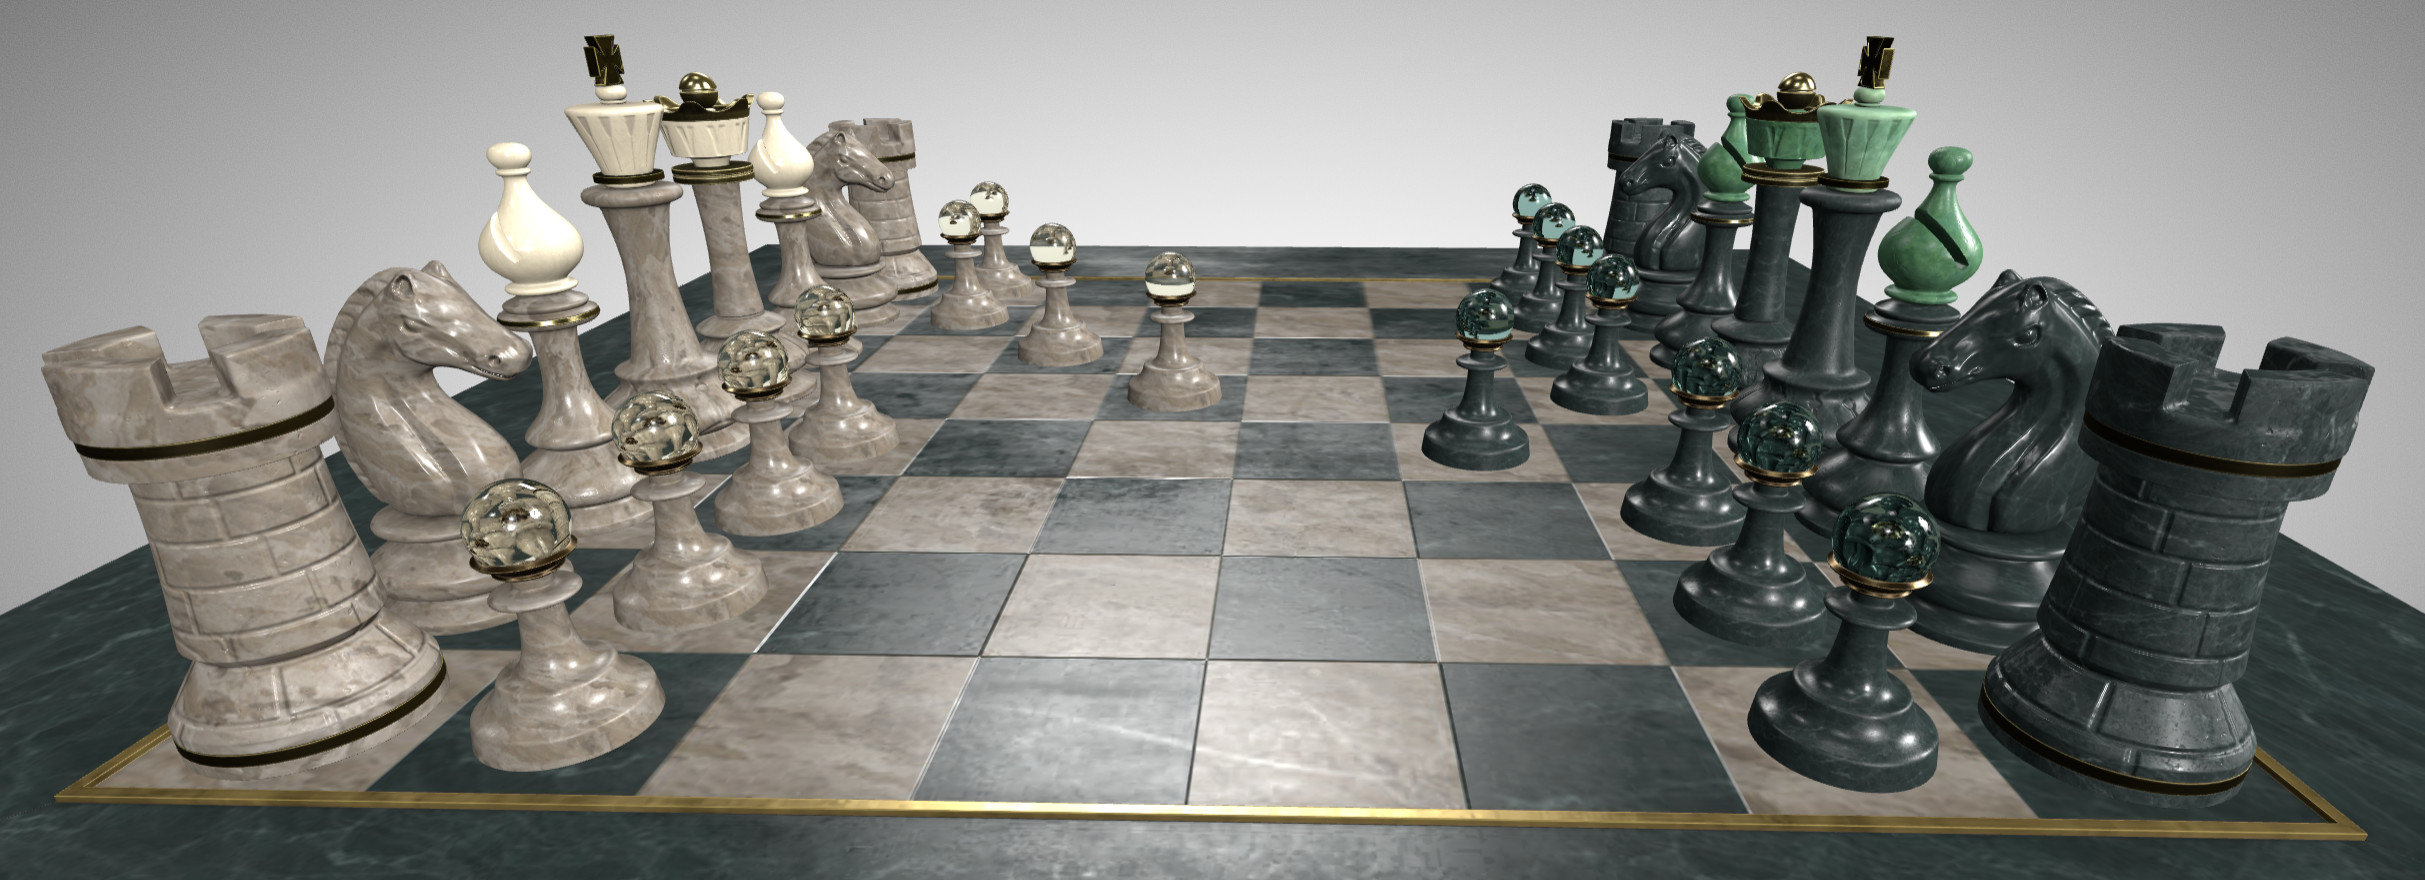
\includegraphics[width=0.8\textwidth]{figuras/a-beautiful-game.jpg}
  \fonte{\citeonline{KhronosSamples2026}}
\end{figure}

\subsection{Geração controlada das versões}

Para a criação das versões modificadas do objeto de teste, utiliza-se um
\textit{script} de modificação especificamente para simular edições típicas
realizadas por um artista sobre a geometria de um modelo. As alterações são
aplicadas diretamente nos valores de ponto flutuante de 32 \textit{bits} contidos
nas \textit{bufferViews} de geometria do arquivo \texttt{ABeautifulGame.glb}. Essa
abordagem garante que as modificações mimetizem de forma realista as alterações
incrementais que ocorrem em um fluxo de trabalho de modelagem tridimensional.

A reprodutibilidade dos experimentos é assegurada pela utilização de uma semente
fixa para o gerador de números pseudoaleatórios. Este procedimento garante que as
sequências de modificações aplicadas sejam idênticas em ambos os ambientes de teste,
permitindo uma comparação direta e justa entre a abordagem proposta e o método de
referência. A consistência na geração das versões é fundamental para validar a
eficácia dos mecanismos de versionamento em cenários controlados.

O experimento considera oito cenários de teste, cada um representando uma
intensidade crescente de modificação, variando de 2\% a 90\% dos dados de geometria.
A progressão gradual da intensidade das alterações permite observar o comportamento
do método em diversas condições, desde edições pontuais e localizadas até
modificações massivas que afetam grande parte da estrutura do modelo. A
Tabela~\ref{tab:cenarios} detalha os cenários e suas respectivas intensidades de
modificação.

\begin{table}[htb]
  \centering
  \caption{\label{tab:cenarios}Cenários de teste e intensidades de modificação}
  \begin{tabular}{cc}
    \toprule
    \textbf{Cenário} & \textbf{Intensidade de modificação} \\
    \midrule
    1 & 2\%  \\
    2 & 5\%  \\
    3 & 10\% \\
    4 & 20\% \\
    5 & 30\% \\
    6 & 50\% \\
    7 & 70\% \\
    8 & 90\% \\
    \bottomrule
  \end{tabular}
  \fonte{Autoria própria (2026)}
\end{table}

\subsection{Método proposto}

O mecanismo de versionamento desenvolvido possui duas camadas complementares. Na
camada lógica, ilustrada na Figura~\ref{fig:fluxo-glb}, um módulo de análise
implementado em Python realiza a leitura e a decomposição do arquivo \gls{glb}. Na
camada física, o sistema de arquivos \gls{btrfs} é responsável pelo armazenamento
diferencial e pela preservação das versões anteriores por meio de
\textit{snapshots} baseados no mecanismo \gls{cow}.

A árvore correspondente ao primeiro \textit{snapshot} é composta pela raiz inicial,
pelos nós internos e pelos nós folha contendo as \textit{bufferViews} originais.
Após o registro de uma nova versão contendo uma modificação, quando o sistema
detecta a alteração de uma \textit{bufferView}, como por exemplo a
\texttt{bv\_0011}, o mecanismo \gls{cow} do \gls{btrfs} aloca um novo nó folha
\texttt{bv\_0011$'$} para armazenar o conteúdo atualizado, sem sobrescrever o bloco
original. Como a modificação afeta apenas um ramo da árvore, o nó interno A precisa
ser copiado para um novo nó A$'$, cujo ponteiro é atualizado para referenciar
\texttt{bv\_0011$'$} em vez de \texttt{bv\_0011}. Esse processo de cópia
propaga-se até a raiz, resultando em uma nova raiz que representa o estado do
segundo \textit{snapshot}.

É importante destacar que isso não representa a criação de uma segunda árvore
completa: apenas os nós no caminho entre o nó modificado e a raiz recebem cópias
novas. Todos os demais nós continuam existindo uma única vez no disco,
compartilhados entre os dois \textit{snapshots} sem qualquer duplicação. O nó
interno B e todos os nós folha sob seu ramo, incluindo \texttt{bv\_0020},
\texttt{bv\_0024} e os demais, permanecem intocados e são referenciados
simultaneamente pelos dois \textit{snapshots}. Por consequência, o custo de
armazenamento do \textit{snapshot} \texttt{v0002} é proporcional exclusivamente ao
volume de dados que efetivamente se altera. O novo nó folha, o nó interno copiado e
a nova raiz, correspondendo a uma fração mínima do tamanho total do arquivo.

Após a compreensão do funcionamento das duas camadas, definem-se as etapas gerais do
método. A primeira etapa consiste na leitura do contêiner \gls{glb} e em sua
separação em pedaços. Conforme descrito na Seção~\ref{sec:LABEL-GLB}, o formato
\gls{glb} organiza seu conteúdo em um \gls{json}, responsável pela descrição da
estrutura da cena, e um arquivo binário, que armazena os dados brutos. O módulo de
análise lê o cabeçalho de 12 \textit{bytes} do arquivo, identifica as porções do
arquivo por seus identificadores de tipo e as separa em memória para processamento
nas etapas seguintes.

A segunda etapa consiste na extração das \textit{bufferViews} como unidades de
versionamento. Como apresentado na Seção~\ref{sec:LABEL-JSON}, o \gls{json} do
\gls{gltf} descreve cada \textit{bufferView} por meio de um par de valores,
\texttt{byteOffset} e \texttt{byteLength}, que delimita com precisão a posição e o
tamanho de cada segmento dentro do binário. Sendo assim, o módulo extrai cada
\textit{bufferView} individualmente, produzindo unidades de dados semanticamente
conexas e independentes entre si.

O terceiro passo envolve a criação de uma assinatura digital única para cada
\textit{bufferView}. O algoritmo \gls{sha256} é aplicado sobre os \textit{bytes} de
cada segmento, produzindo um identificador de 256 \textit{bits} que representa
exclusivamente o conteúdo daquela unidade. Esses \textit{hashes} são armazenados em
arquivo \gls{json} ao término de cada operação de versionamento, constituindo o
estado de referência utilizado na comparação com a versão subsequente.

A quarta etapa é crucial para o estado lógico do método, consistindo na detecção
diferencial entre versões. Ao receber um novo arquivo \gls{glb}, o sistema extrai
suas \textit{bufferViews}, calcula os \textit{hashes} correspondentes e os compara
com os da versão anterior. Nesse sentido, cada \textit{bufferView} é classificada em
uma de quatro categorias: nova, modificada, removida ou inalterada. Apenas as
classificadas como novas ou modificadas são encaminhadas para gravação em disco. As
\textit{bufferViews} inalteradas são descartadas do processo de escrita, pois seus
dados já estão preservados no subvolume ativo.

A quinta etapa consiste na gravação dos segmentos modificados no subvolume
\gls{btrfs} e na criação de um \textit{snapshot} imutável. Cada \textit{bufferView}
é armazenada como um arquivo binário independente no subvolume ativo, identificado
pelo seu índice no arquivo \gls{glb}. Após a gravação dos segmentos modificados, o
mecanismo nativo de \textit{snapshots} do \gls{btrfs} é acionado para registrar o
estado atual do subvolume como uma versão imutável de leitura. Conforme discutido
nas Seções~\ref{sec:LABEL-COW} e \ref{sec:LABEL-BTRFS}, o \gls{btrfs} implementa
esse mecanismo por meio do modelo \gls{cow}, no qual os blocos físicos não
modificados entre versões consecutivas são compartilhados entre o subvolume ativo e
os \textit{snapshots} anteriores, sem duplicação de dados no disco. Dessa forma, o
custo de armazenamento de cada \textit{snapshot} é proporcional exclusivamente ao
volume de dados efetivamente alterado, e não ao tamanho total do arquivo versionado.

\subsection{Conceitos Fundamentais da Camada Física}

A camada física do método proposto é fundamentada no sistema de arquivos
\gls{btrfs}, como pode-se observar na subseção anterior, escolhido por sua
capacidade avançada de gerenciamento de dados e versionamento.

Um dos pilares do \gls{btrfs} são os subvolumes. Diferente de um diretório comum, um
subvolume é uma unidade independente que possui sua própria árvore de dados. Isso
significa que ele pode ser tratado como um sistema de arquivos separado, mesmo
estando dentro de um volume \gls{btrfs} maior. No método acima, utiliza-se
subvolumes para organizar o ciclo de versionamento. Um subvolume principal, este
chamado versões, atua como um contêiner, e dentro dele, um subvolume ativo, chamado
versão atual, representa a área de trabalho onde os dados das \textit{bufferViews}
são gravados e atualizados.

A eficiência do \gls{btrfs} no versionamento é alcançada pela combinação entre o
modelo \gls{cow} e sua organização interna baseada em árvores-B. Diferentemente de
sistemas de arquivos tradicionais, que mantêm estruturas de metadados em posições
fixas do disco, o \gls{btrfs} organiza todo o seu estado persistente, sendo composto
por arquivos, diretórios, extensões de dados e \textit{checksums}, em um conjunto de
árvores-B aninhadas, todas enraizadas em uma estrutura central denominada árvore
raiz. Cada nó interno dessas árvores armazena chaves de busca e ponteiros para os
nós filhos, enquanto os nós folha contêm os dados ou metadados propriamente ditos.
Essa organização hierárquica permite localizar qualquer item do sistema de arquivos
com custo logarítmico em relação ao volume total de dados, tornando as operações de
leitura e escrita eficientes mesmo em volumes de grande escala.

A escolha da árvore-B como estrutura fundamental não é aleatória, sendo essencial
para que o \gls{cow} possa ser implementado de forma eficiente. Quando um bloco de
dados é modificado, o \gls{btrfs} precisa atualizar não apenas o bloco em si, mas
também o caminho de metadados que leva até ele, desde o nó folha até a raiz da
árvore. Em uma estrutura de árvore-B, esse caminho é limitado em profundidade, o que
significa que a propagação da atualização envolve um número controlado de nós. Cada
nó desse caminho recebe uma nova cópia modificada, gravada em uma posição diferente
do disco, enquanto as versões anteriores permanecem intactas. Ao término da
operação, apenas o ponteiro raiz é atualizado para referenciar a nova versão da
árvore. Esse mecanismo, conhecido como \textit{shadow paging}\footnote{\textit{Shadow
paging}, técnica de gerenciamento de escrita que grava modificações em novas páginas
em vez de sobrescrever os blocos originais, atualizando o sistema de forma atômica
ao trocar o ponteiro da raiz da árvore \cite{Rodeh2007}.} na literatura de sistemas
de arquivos, garante que o estado anterior da árvore continue acessível enquanto o
novo estado é construído de forma atômica \cite{Rodeh2007}.

Os \textit{snapshots} são uma consequência direta dessa arquitetura. Como o estado
completo de um subvolume é representado por um único ponteiro raiz, criar um
\textit{snapshot} equivale a registrar uma referência adicional para essa raiz em um
momento específico. \textit{Snapshot} e subvolume ativo passam a compartilhar todos
os nós da árvore existentes no instante da captura. À medida que novas modificações
são aplicadas ao subvolume ativo, apenas os nós efetivamente alterados e seus
ancestrais recebem cópias novas no disco, enquanto os nós inalterados continuam
sendo referenciados por ambas as versões simultaneamente. Configurados com o
argumento \texttt{-r}, os \textit{snapshots} tornam-se somente leitura, o que impede
qualquer atualização posterior sobre aquela raiz e garante a imutabilidade do estado
registrado. É exatamente esse comportamento que fundamenta a estratégia de
versionamento proposta neste estudo, sendo assim, ao gravar no subvolume ativo
apenas as \textit{bufferViews} classificadas como modificadas ou novas, e em seguida
capturar um \textit{snapshot} imutável, o sistema garante que o custo de
armazenamento de cada versão seja proporcional exclusivamente ao volume de dados que
efetivamente se altera.

\subsection{Método de referência configurado como \gls{gitlfs}}

O método de referência utiliza um repositório Git local, configurado com o
\gls{gitlfs}, na instância \texttt{tcc-gitlfs}. Ele funciona através de ganchos que
são ativados durante as operações do Git. Estes que, redirecionam os arquivos
grandes para um armazenamento especial, fora do histórico principal. A configuração
para rastrear arquivos \gls{glb} com \gls{lfs} é feita no arquivo
\texttt{.gitattributes}, onde é estipulado uma regra que indica que todos os
arquivos com essa extensão devem ser tratados como objetos grandes.

Cada operação de versionamento começa com a cópia do arquivo \gls{glb} modificado
para o diretório do repositório. Em seguida, o comando \texttt{git add} é executado.
Neste ponto, o gatilho do \gls{gitlfs} entra em ação, ele lê o arquivo \gls{glb}
completo, calcula seu \textit{hash} e armazena o arquivo binário no diretório
\texttt{.git/lfs/objects}. Esse diretório é organizado em subdiretórios baseados nos
primeiros \textit{bytes} do \textit{hash} para facilitar a localização. No lugar do
arquivo \gls{glb} original, o Git armazena apenas um pequeno arquivo de ponteiro,
com cerca de 130 \textit{bytes}. Este ponteiro contém informações como o algoritmo
de \textit{hash} usado, o identificador do objeto \gls{lfs} e o tamanho original do
arquivo. É esse arquivo de ponteiro que é, de fato, versionado pelo Git, enquanto o
conteúdo real do arquivo grande permanece no armazenamento do \gls{lfs}.

A etapa seguinte é o \texttt{git commit}, que registra o arquivo de ponteiro no
histórico do repositório, como faria com qualquer outro arquivo de texto. No
entanto, o \gls{gitlfs} não utiliza conceitos como subvolumes, \textit{snapshots} ou
compartilhamento de blocos entre versões, que são característicos de sistemas como o
\gls{btrfs}. Cada objeto armazenado no \gls{lfs} é um arquivo binário completo e
independente. A única forma de economia de espaço é a deduplicação por
\textit{hash}, que acontece quando duas versões de um arquivo resultam no mesmo
\textit{hash}, o \gls{lfs} não cria um segundo objeto. Fora essa situação, que
ocorre apenas quando o arquivo não sofreu nenhuma alteração, cada nova versão
adiciona uma cópia integral do arquivo ao armazenamento do \gls{lfs},
independentemente da quantidade de dados que é modificada em relação à versão
anterior.

Para este experimento, isso significa que cada um dos nove cenários de teste, mesmo
com pequenas modificações, resulta na adição de aproximadamente 42,9 MB ao diretório
\texttt{.git/lfs/objects}. O crescimento do armazenamento do \gls{lfs} é, portanto,
linear em relação ao número de versões registradas, sem considerar o volume de dados
que realmente mudou.

\subsection{Métricas de avaliação}

Para comparar o desempenho do método proposto com o método de referência, utiliza-se
métricas que medem o impacto direto das operações de versionamento no disco. Essas
métricas são coletadas de forma padronizada em ambos os ambientes, permitindo uma
comparação justa e direta, independentemente de como cada método funciona
internamente.

A primeira métrica é a quantidade de \textit{bytes} gravados por versão. Ela
representa o volume de dados que é efetivamente escrito no disco quando uma nova
versão é registrada. No método proposto, esse valor é a soma dos tamanhos de todas
as \textit{bufferViews} que foram classificadas como novas ou modificadas.
Matematicamente, isso pode ser expresso como:

\begin{equation}
  \label{eq:bytes-gravados}
  B_{gravados} = \sum tamanho(bv_i), \text{ para todo } bv_i \text{ novo ou modificado}
\end{equation}

Já no método de referência, usando o \gls{gitlfs}, essa métrica corresponde ao
tamanho do novo objeto binário que é adicionado ao diretório de armazenamento das
versões. Isso é medido pela diferença no tamanho total desse armazenamento antes e
depois de cada \textit{commit}. Em ambos os casos, essa métrica nos mostra o custo
imediato de armazenamento para cada operação de versionamento.

A segunda métrica é a \textbf{economia percentual}. Ela mede o quanto de dados não
precisou ser gravado em disco em relação ao tamanho total do arquivo original. É
expressa em porcentagem e calculada da seguinte forma:

\begin{equation}
  \label{eq:economia}
  E = \left( 1 - \frac{B_{gravados}}{B_{total}} \right) \times 100
\end{equation}

Onde $B_{total}$ é o tamanho completo do arquivo \gls{glb}. Esta métrica é
importante porque quantifica o ganho de eficiência do método proposto. No
\gls{gitlfs}, o valor de $B_{gravados}$ geralmente é muito próximo de $B_{total}$,
resultando em uma economia percentual próxima de zero. No método proposto,
presume-se que a economia aumente à medida que a quantidade de modificações no
arquivo diminui, pois mais blocos de dados podem ser compartilhados entre as
versões.

A terceira métrica é o \textbf{armazenamento acumulado}. Ela representa o espaço
total ocupado no disco após o registro de todas as versões ao longo do experimento.

\begin{equation}
  \label{eq:acumulado}
  A_{acumulado} = \sum_{i=1}^{N} B_{gravados}(v_i)
\end{equation}

No método proposto, esse valor é obtido usando o comando \texttt{btrfs filesystem
usage}, que informa o espaço físico real ocupado no volume, já considerando o
compartilhamento de blocos entre os \textit{snapshots}. No método de referência, é o
tamanho total do diretório que armazena os arquivos binários. Embora sejam coletados
de locais diferentes, ambos os valores representam a mesma coisa, o espaço total em
disco usado pelo histórico completo de versões do arquivo. A comparação entre eles é
direta, e a diferença esperada entre os dois métodos mostrará a capacidade do método
proposto de reutilizar blocos físicos entre versões consecutivas, gerando economia
de espaço.

\section{Usando o método em áreas individuais}

O segundo experimento aprofunda a avaliação do mecanismo de versionamento
diferencial, focando na variação da quantidade de \textit{bufferViews} modificadas,
em contraste com a variação da intensidade numérica em todas as
\textit{bufferViews} de geometria empregada no primeiro experimento. O objetivo foi
analisar o impacto da granularidade das alterações no consumo de armazenamento,
novamente em comparação com o \gls{gitlfs}. Para isso, o modelo
\texttt{ABeautifulGame.glb}, composto por 75 \textit{bufferViews} de atributos de
vértice, é submetido a uma série de novas modificações controladas.

Os cenários de teste são definidos para simular um espectro de alterações, desde
modificações mínimas até uma deformação generalizada do modelo. A
Tabela~\ref{tab:cenarios-exp2} apresenta a progressão das versões. Temos uma baixa
mudança dentro de cada pedaço, que garante que as deformações visuais sejam sutis,
mas suficientes para alterar o \textit{hash} \gls{sha256} de cada
\textit{bufferView} modificada, acionando o mecanismo diferencial do sistema. As
\textit{bufferViews} de índices de face são preservadas intactas, evitando a
corrupção de dados.

O segundo experimento aprofunda a avaliação do mecanismo de versionamento
diferencial, focando na variação da quantidade de \textit{bufferViews} modificadas,
em contraste com a variação da intensidade numérica em todas as
\textit{bufferViews} de geometria empregada no primeiro experimento. O objetivo foi
analisar o impacto da granularidade das alterações no consumo de armazenamento,
novamente em comparação com o \gls{gitlfs}. Para isso, o modelo
\texttt{ABeautifulGame.glb}, composto por 75 \textit{bufferViews} de atributos de
vértice, é submetido a uma série de novas modificações controladas.

Os cenários de teste são definidos para simular um espectro de alterações, desde
modificações mínimas até uma deformação generalizada do modelo. A
Tabela~\ref{tab:cenarios-exp2} apresenta a progressão das versões. Temos uma baixa
mudança dentro de cada pedaço, que garante que as deformações visuais sejam sutis,
mas suficientes para alterar o \textit{hash} \gls{sha256} de cada
\textit{bufferView} modificada, acionando o mecanismo diferencial do sistema. As
\textit{bufferViews} de índices de face são preservadas intactas, evitando a
corrupção de dados.

\begin{table}[htb]
  \centering
  \caption{\label{tab:cenarios-exp2}Cenários de teste e progressão de modificação por bufferView em áreas individuais}
  \begin{tabular}{ccc}
    \toprule
    \textbf{Versão} & \textbf{Porcentagem modificada} & \textbf{Quantidade modificada} \\
    \midrule
    v1 & linha de base & 0  \\
    v2 & 1\%           & 1  \\
    v3 & 5\%           & 4  \\
    v4 & 10\%          & 8  \\
    v5 & 25\%          & 19 \\
    v6 & 50\%          & 38 \\
    v7 & 75\%          & 57 \\
    v8 & 100\%         & 75 \\
    \bottomrule
  \end{tabular}
  \fonte{Autoria própria (2026)}
\end{table}

Para a implementação deste experimento, o método para gerar as modificações nos
arquivos é adaptado com duas mudanças fundamentais. Primeiramente, é implementada a
separação das \textit{bufferViews} de índices dos atributos, garantindo que apenas
os dados de ponto flutuante sejam modificados, evitando a corrupção de índices de
face. Em segundo lugar, o \textit{script} passa a aceitar a quantidade de
\textit{bufferViews} a modificar como parâmetro, em vez de um tipo genérico de
modificação. Essas adaptações permitem um controle preciso sobre a granularidade das
alterações, essencial para a validação da eficiência do versionamento por blocos em
termos de economia de armazenamento, especialmente quando comparado a métodos que
não exploram a estrutura interna dos arquivos \gls{glb}.

\section{Cronograma de desenvolvimento}

O desenvolvimento do trabalho será organizado em \textit{sprints} de duas semanas,
seguindo os princípios de desenvolvimento iterativo, nos quais cada ciclo possui um
objetivo claro e entregável. O período de execução compreende os meses de agosto a
novembro de 2026, totalizando sete \textit{sprints}.

\begin{enumerate}
  \item \textbf{Agosto, semanas 1 e 2:} a primeira \textit{sprint} tem como objetivo
  a consolidação da arquitetura de versionamento. Implementam-se as operações
  fundamentais de recuperação automática de versões anteriores e o registro
  estruturado do histórico, substituindo a interação direta com o terminal por uma
  interface programática mais acessível e reproduzível.

  \item \textbf{Agosto, semanas 3 e 4:} a segunda \textit{sprint} é dedicada ao
  estudo e à prototipação de estratégias de fusão entre versões. Analisam-se as
  possibilidades de combinar \textit{bufferViews} modificadas em paralelo,
  identificando cenários de conflito e definindo o comportamento esperado do sistema
  diante dessas situações.

  \item \textbf{Setembro, semanas 1 e 2:} a terceira \textit{sprint} concentra-se na
  integração do método proposto com um \textit{software} de edição tridimensional. O
  objetivo é desenvolver um mecanismo que permita acionar o versionamento
  diretamente a partir do fluxo de trabalho do desenvolvedor, sem necessidade de
  interação manual com o terminal, tornando a solução utilizável em um ambiente de
  produção real.

  \item \textbf{Setembro, semanas 3 e 4:} a quarta \textit{sprint} abrange o estudo
  de viabilidade e a prototipação inicial de uma camada \textit{web} sobre a base de
  versionamento existente. Definem-se a arquitetura de requisições e as operações
  básicas que permitirão ao sistema operar de forma distribuída, saindo do
  repositório estritamente local.

  \item \textbf{Outubro, semanas 1 e 2:} a quinta \textit{sprint} dá continuidade ao
  desenvolvimento do protótipo \textit{web}, consolidando as operações de envio,
  recuperação e listagem de versões. Ao término desta \textit{sprint} contempla a
  validação da viabilidade técnica da abordagem distribuída.

  \item \textbf{Outubro, semanas 3 e 4:} a sexta \textit{sprint} é destinada à
  execução dos experimentos finais e à coleta dos resultados com a arquitetura
  completa. Os cenários de teste repetem-se considerando as novas funcionalidades
  implementadas, e os dados obtidos fundamentaram a elaboração da seção de
  resultados e da discussão final do trabalho.

  \item \textbf{Novembro, semanas 1 e 2:} a sétima e última \textit{sprint}
  compreende a revisão geral do texto, a escrita da conclusão, a elaboração da
  documentação técnica da arquitetura final e a preparação da apresentação para a
  banca avaliadora.
\end{enumerate}

